\documentclass [11pt, a4wide, twoside]{article}

\usepackage{times}
\usepackage{epsfig}
\usepackage{ifthen}
\usepackage{xspace}
\usepackage{fancyhdr}
\usepackage[colorlinks,urlcolor=blue]{hyperref}
\usepackage{verbatim}
\usepackage{amsmath}
\usepackage{amssymb}
\usepackage{graphicx}

\usepackage{listings}
\usepackage{color}

\definecolor{dkgreen}{rgb}{0,0.6,0}
\definecolor{gray}{rgb}{0.5,0.5,0.5}
\definecolor{mauve}{rgb}{0.58,0,0.82}

\lstset{frame=tb,
  language=Java,
  aboveskip=3mm,
  belowskip=3mm,
  showstringspaces=false,
  columns=flexible,
  basicstyle={\small\ttfamily},
  numbers=none,
  numberstyle=\tiny\color{gray},
  keywordstyle=\color{blue},
  commentstyle=\color{dkgreen},
  stringstyle=\color{mauve},
  breaklines=true,
  breakatwhitespace=true
  tabsize=3
}

% solution switch
\newboolean{showsolution}
\setboolean{showsolution}{true} 

\usepackage{times}
\usepackage{epsfig}
\usepackage{ifthen}
\usepackage{xspace}
\usepackage{fancyhdr}
\usepackage{amsthm}
\usepackage{hyperref}



%layout
\topmargin      -5.0mm
\oddsidemargin  6.0mm
\evensidemargin -6.0mm
\textheight     215.5mm
\textwidth      160.0mm
\parindent      1.0em
\headsep        10.3mm
\headheight     12pt
\lineskip       1pt
\normallineskip 1pt

\newtheorem{mydef}{Definition}


%header
\lhead{Software Modeling and Analysis \\ 2016}

\rhead{Prof. Oscar Nierstrasz, Mohammad Ghafari, Nevena Milojkovi\'{c} and Yuriy Tymchuk}

\lfoot{page \thepage}
\rfoot{\today}
\cfoot{}

\renewcommand{\headrulewidth}{0.1pt}
\renewcommand{\footrulewidth}{0.1pt}

%enumeration
\newenvironment{myitemize}{%
     \begin{itemize}
     \setlength{\itemsep}{0cm}}
     {\end{itemize}}

\newenvironment{myenumerate}{%
     \begin{enumerate} \setlength{\itemsep}{0cm}}
     {\end{enumerate}}


%solution
\ifthenelse{\boolean{showsolution}}
   {  \newcommand{\solution}[1]{
   	\noindent\underline{\textbf{Answer:}}\\[2mm]
   	 \textsl{#1}
	 \vspace{10pt}
	 \normalsize
	}
  }
  {  \newcommand{\solution}[1]{} }


\pagestyle{fancy}

% ============================================================
% Markup macros for proof-reading
\usepackage{ifthen}
\usepackage[normalem]{ulem} % for \sout
\usepackage{xcolor}
\newcommand{\ra}{$\rightarrow$}
\newboolean{showedits}
\setboolean{showedits}{true} % toggle to show or hide edits
\ifthenelse{\boolean{showedits}}
{
	\newcommand{\ugh}[1]{\textcolor{red}{\uwave{#1}}} % please rephrase
	\newcommand{\ins}[1]{\textcolor{blue}{\uline{#1}}} % please insert
	\newcommand{\del}[1]{\textcolor{red}{\sout{#1}}} % please delete
	\newcommand{\chg}[2]{\textcolor{red}{\sout{#1}}{\ra}\textcolor{blue}{\uline{#2}}} % please change
}{
	\newcommand{\ugh}[1]{#1} % please rephrase
	\newcommand{\ins}[1]{#1} % please insert
	\newcommand{\del}[1]{} % please delete
	\newcommand{\chg}[2]{#2}
}
% ============================================================
% Put edit comments in a really ugly standout display
%\usepackage{ifthen}
\usepackage{amssymb}
\newboolean{showcomments}
\setboolean{showcomments}{true}
%\setboolean{showcomments}{false}
\newcommand{\id}[1]{$-$Id: scgPaper.tex 32478 2010-04-29 09:11:32Z oscar $-$}
\newcommand{\yellowbox}[1]{\fcolorbox{gray}{yellow}{\bfseries\sffamily\scriptsize#1}}
\newcommand{\triangles}[1]{{\sf\small$\blacktriangleright$\textit{#1}$\blacktriangleleft$}}
\ifthenelse{\boolean{showcomments}}
%{\newcommand{\nb}[2]{{\yellowbox{#1}\triangles{#2}}}
{\newcommand{\nbc}[3]{
 {\colorbox{#3}{\bfseries\sffamily\scriptsize\textcolor{white}{#1}}}
 {\textcolor{#3}{\sf\small$\blacktriangleright$\textit{#2}$\blacktriangleleft$}}}
 \newcommand{\version}{\emph{\scriptsize\id}}}
{\newcommand{\nbc}[3]{}
 \renewcommand{\ugh}[1]{#1} % please rephrase
 \renewcommand{\ins}[1]{#1} % please insert
 \renewcommand{\del}[1]{} % please delete
 \renewcommand{\chg}[2]{#2} % please change
 \newcommand{\version}{}}
\newcommand{\nb}[2]{\nbc{#1}{#2}{orange}}
\newcommand{\here}{\yellowbox{$\Rightarrow$ CONTINUE HERE $\Leftarrow$}}
\newcommand\rev[2]{\nb{TODO (rev #1)}{#2}} % reviewer comments
\newcommand\fix[1]{\nb{FIX}{#1}}
\newcommand\todo[1]{\nb{TO DO}{#1}}
\newcommand\on[1]{\nbc{ON}{#1}{red}} % add more author macros here
%\newcommand\XXX[1]{\nbc{XXX}{#1}{blue}}
%\newcommand\XXX[1]{\nbc{XXX}{#1}{brown}}
%\newcommand\XXX[1]{\nbc{XXX}{#1}{cyan}}
%\newcommand\XXX[1]{\nbc{XXX}{#1}{darkgray}}
%\newcommand\XXX[1]{\nbc{XXX}{#1}{gray}}
%\newcommand\XXX[1]{\nbc{XXX}{#1}{magenta}}
%\newcommand\XXX[1]{\nbc{XXX}{#1}{olive}}
%\newcommand\XXX[1]{\nbc{XXX}{#1}{orange}}
%\newcommand\XXX[1]{\nbc{XXX}{#1}{purple}}
%\newcommand\XXX[1]{\nbc{XXX}{#1}{red}}
%\newcommand\XXX[1]{\nbc{XXX}{#1}{teal}}
%\newcommand\XXX[1]{\nbc{XXX}{#1}{violet}}
%=============================================================
% ST80 listings macros
% Adapted from Squeak by Example book
%=============================================================
% If you want >>> appearing as right guillemet, you need these two lines:
%\usepackage[T1]{fontenc}
%\newcommand{\sep}{\mbox{>>}}
% Otherwise use this:
\newcommand{\sep}{\mbox{$\gg$}}
%=============================================================
%:\needlines{N} before code block to force page feed
\usepackage{needspace}
\newcommand{\needlines}[1]{\Needspace{#1\baselineskip}}
%=============================================================
%:Listings package configuration for ST80
\usepackage[english]{babel}
\usepackage{amssymb,textcomp}
\usepackage{listings}
% \usepackage[usenames,dvipsnames]{color}
% \usepackage[usenames]{color}
% \definecolor{source}{gray}{0.95}
\lstdefinelanguage{Smalltalk}{
%  morekeywords={self,super,true,false,nil,thisContext}, % This is overkill
  morestring=[d]',
  morecomment=[s]{"}{"},
  alsoletter={\#:},
  escapechar={!},
  literate=
    {BANG}{!}1
    {UNDERSCORE}{\_}1
    {\\st}{Smalltalk}9 % convenience -- in case \st occurs in code
    % {'}{{\textquotesingle}}1 % replaced by upquote=true in \lstset
    {_}{{$\leftarrow$}}1
    {>>>}{{\sep}}1
    {^}{{$\uparrow$}}1
    {~}{{$\sim$}}1
    {-}{{\sf -\hspace{-0.13em}-}}1  % the goal is to make - the same width as +
    {+}{\raisebox{0.08ex}{+}}1		% and to raise + off the baseline to match -
    {-->}{{\quad$\longrightarrow$\quad}}3
	, % Don't forget the comma at the end!
  tabsize=4
}[keywords,comments,strings]

\definecolor{source}{gray}{0.95}

\lstset{language=Smalltalk,
	basicstyle=\sffamily,
	keywordstyle=\color{black}\bfseries,
	% stringstyle=\ttfamily, % Ugly! do we really want this? -- on
	mathescape=true,
	showstringspaces=false,
	keepspaces=true,
	breaklines=true,
	breakautoindent=true,
	backgroundcolor=\color{source},
	lineskip={-1pt}, % Ugly hack
	upquote=true, % straight quote; requires textcomp package
	columns=fullflexible} % no fixed width fonts
% In-line code (literal)
% Normally use this for all in-line code:
\newcommand{\ct}{\lstinline[mathescape=false,backgroundcolor=\color{white},basicstyle={\sffamily\upshape}]}
% In-line code (latex enabled)
% Use this only in special situations where \ct does not work
% (within section headings ...):
\newcommand{\lct}[1]{{\textsf{\textup{#1}}}}
% Code environments
\lstnewenvironment{code}{%
	\lstset{%
		% frame=lines,
		frame=single,
		framerule=0pt,
		mathescape=false
	}
}{}

% Useful to add a matching $ after code containing a $
% \def\ignoredollar#1{}
%=============================================================
\newcommand{\ie}{\emph{i.e.}\xspace}
\newcommand{\eg}{\emph{e.g.}\xspace}
\newcommand{\etal}{\emph{et al.}\xspace}
% ============================================================


\begin{document}

\section*{\ifthenelse{\boolean{showsolution}}{\textcolor{red}{Solution}\\}{}Assignment 03  --- 30.09.2020 -- v1.0\\Smalltalk: Understanding Classes and Metaclasses}

\textcolor{red}{Please submit this assignment by email to \href{mailto:pascal.gadient@inf.unibe.ch}{pascal.gadient@inf.unibe.ch} \underline{before} 07. October 2020, 10:15am.}

\subsection*{Exercise 1 -- Metamodels (2.5 pts)}
Answer the following questions regarding metamodels:
\begin{enumerate}[i)]

\item What is a metamodel?
\solution{It is a model of a model. In other words, a metamodel is a prescriptive view on an existing model. A metamodel determines the syntax and semantics of models that conform to it. Metamodels can leverage various forms, \eg grammar syntax, flow charts, and UML diagrams.}

\item How are metamodels used in Pharo?\\You must use the classes \texttt{Object}, \texttt{Class}, and \texttt{Metaclass} in your answer.
%\on{Small point. I would say "Pharo" or at best "Pharo/GT", since GT does not add anything to Pharo's object model. Pharo does add traits and slots to the object model of Smalltalk-80, and there are other differences too.}\\
\solution{Every object is an instance of a class. Every class inherits from \texttt{Object}. Every class is an instance of its (unique) metaclass, which inherits from \texttt{Class}. Every metaclass is an instance of \texttt{Metaclass}, which is itself a class.}

%For example, if a user creates a new class it will automatically extend the \texttt{Class} class, the corresponding object instance will automatically extend the \texttt{Object} class, and the corresponding metaclass instance will automatically extend the \texttt{Metaclass} class.
%Every implemented class has a representation that extends the \texttt{Class} class which is accessible at run time and allows reification. Every instance of such an element is }

\item What are responsibilities of a metaclass in Pharo?
\solution{Instance creation, creating initialized instances of the metaclass's sole instance, initialization of class variables, metaclass instance protocol, method compilation (different semantics can be introduced), class information (inheritance link, instance variable, ...).}

\item Where is \texttt{ProtoObject} located in Pharo's class hierarchy?
\solution{In Pharo, \texttt{ProtoObject} is the root class for all other classes including \texttt{Object}. \texttt{ProtoObject} is the superclass of \texttt{Object}.}

\item What is the purpose of the class \texttt{ProtoObject}?
\solution{While \texttt{Object} provides (most of) the common message handlers, \eg \texttt{printOn}, the class \texttt{ProtoObject} does not carry all that ``baggage'' and only contains the core behavior needed to make the system work.
The idea of \texttt{ProtoObject} is to have a lean class that separates the concerns.}
%Additionally provides objects some ``x-ray'' capabilities for developers who are working on the GT VM, and enables the use of more advanced features like metaclass operations.
%Consequently, although it is not very well known, \texttt{ProtoObject} is heavily used as it offers convenient method receivers, \eg for debugging, introspection, or memory scanning.
%\on{OK, but the main point is that Object has a large number of methods. The idea of ProtoObject is to have a lean class that does not carry all this baggage. It contains only the core behaviour needed to make the system work. I would not say that ProtoObjects "adds a layer of abstraction".}


\end{enumerate}
%Pooja question:
%I think asking advantage and disadvantages of Live systems in contrast to traditional systems, would be easier to ask. In the end, the answer you are expecting (threat) is a type of disadvantage.
%Also, students would not able to reach the example, "For instance, GT will crash" until you ask them to provide a situation where live systems are in a disadvantage.
%b) In addition to what a message is, it would be nice to add, what are the types of messages in Smalltalk.
%ans: There are three types of messages, Unary, binary and keyword messages.

\vspace{1.5cm}

\ifthenelse{\boolean{showsolution}}{}{\begin{center}\center{\large{\emph{\textbf{Please continue reading on the next page.}}}\newpage}\end{center}}

\subsection*{Exercise 2 -- Sub and super classes (3 pts)}
Answer the questions below.
Please provide your code \emph{\underline{and}} your results.
\begin{enumerate}[i)]

\item How many superclasses does \texttt{Collection} have?
\solution{\texttt{Collection allSuperclasses size.}\\2. Consequently, the class has two super classes.}

\item How many direct subclasses does \texttt{Collection} have?
\solution{\texttt{Collection subclasses size.}\\32. Therefore, the class has 32 direct subclasses.}

\item How many indirect subclasses does \texttt{Collection} have?
\solution{\texttt{Collection allSubclasses size - Collection subclasses size.}\\129. The class \texttt{Collection} has a total of 161 subclasses, whereas (161 - 32 =) 129 are indirect subclasses.}
%In GT, even more metrics are directly accessible, \eg the total lines of code:\\
%\texttt{Collection linesOfCode.} which would yield 1087.}
\end{enumerate}
\emph{NB: Direct subclasses are classes that extend a base class directly (\eg relation parents to children), whereas indirect subclasses extend the direct and (recursively) indirect subclasses (\eg relation grandparents to grandchildren).}\\\\
\emph{NB: Please use a fresh copy of GT.}

\vspace{1.5cm}
\ifthenelse{\boolean{showsolution}}{\newpage}{}

\subsection*{Exercise 3 -- Class identity (3 pts)}
\begin{figure}[h]
\centering
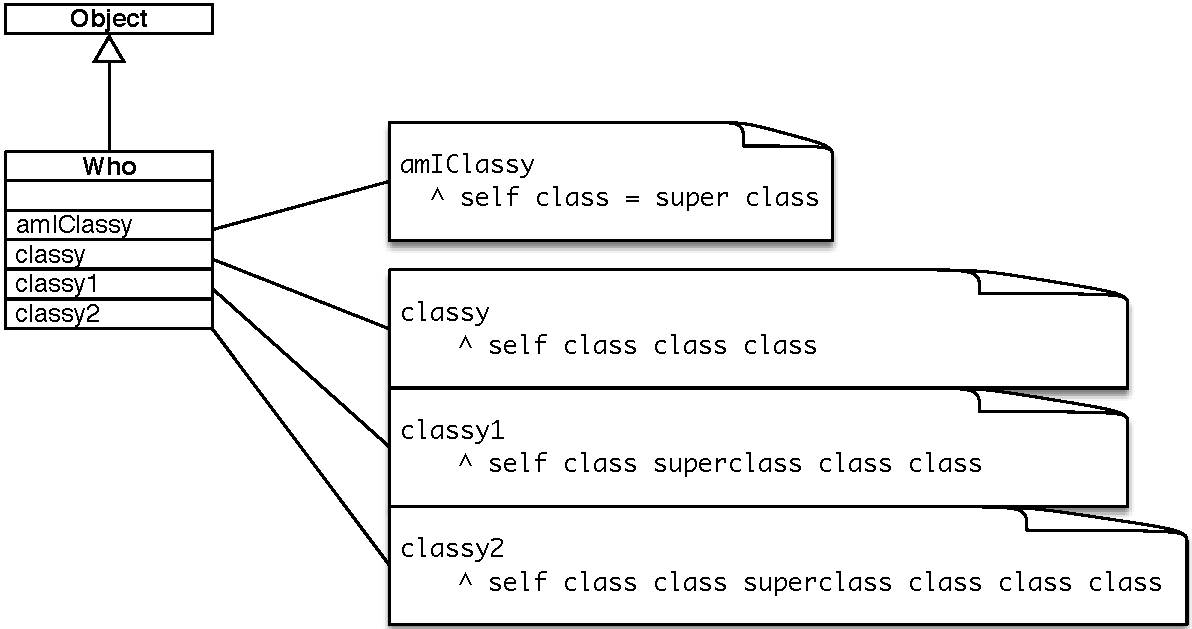
\includegraphics[width=0.7\textwidth]{super.pdf}
\end{figure}
\noindent

%Pooja question:
%I think asking advantage and disadvantages of Live systems in contrast to traditional systems, would be easier to ask. In the end, the answer you are expecting (threat) is a type of disadvantage.
%Also, students would not able to reach the example, "For instance, GT will crash" until you ask them to provide a situation where live systems are in a disadvantage.
%b) In addition to what a message is, it would be nice to add, what are the types of messages in Smalltalk.
%ans: There are three types of messages, Unary, binary and keyword messages.

\noindent Consider the implementation shown in the illustration.\\

\noindent What are the results (either \texttt{true} or \texttt{false}) of the following statements?\\
Explain for each statement why GT replied the corresponding result.
\begin{enumerate}[a)]

\item \texttt{Who new amIClassy.}
\solution{True. \texttt{super} is executed in the context of the class of the method implementation. \texttt{super class} starts the lookup in the superclass of the implementing method, namely \texttt{Object}, while \texttt{self class} starts in the class of the instance, namely \texttt{Who}. But since \texttt{Who} does not implement class, both expressions find the same method.}

\item \texttt{Who new classy = Who new classy1.}
\solution{True. Both call chains reach the root of the class hierarchy tree (Metaclass class) which is identical for both of them.\newline
\texttt{Who new classy}: \texttt{Who class class class}, returns a \texttt{Metaclass class}.\newline
\texttt{Who new classy1}: \texttt{Who class superclass} returns an \texttt{Object class}, \texttt{Object class class class} finally returns a \texttt{Metaclass class}.}

\item \texttt{Who new classy1 = Who new classy2.}
\solution{True. Both elements represent the same class.\newline
\texttt{Who new classy1}: Returns a \texttt{Metaclass class}.\newline
\texttt{Who new classy2}: \texttt{self class class} returns a \texttt{Metaclass (Who class)} object, \\\texttt{Metaclass (Who class) superclass} returns a \texttt{Metaclass (Object class)} object, and finally, \texttt{Metaclass (Object class) class class class} returns a \texttt{Metaclass class}. The last two message sends exploit the circular dependency between \texttt{Metaclass} and the \texttt{Metaclass class}.}
\end{enumerate}

%\subsection*{Exercise 2 -- Abstract methods (1.5 pts)}
%Find all abstract methods of the class \texttt{Collection}.\\ \newline
%\emph{Hints: An abstract method has the body \texttt{self subclassResponsibility}, and you should use the messages \texttt{allMethods}, \texttt{select}, and \texttt{isAbstract}.}
%Use the message \texttt{methods} to retrieve all methods of a class, and then send \texttt{messages} to retrieve all messages sent by a specific method.}
%\solution{\texttt{Collection methods select: [:eachMethod | eachMethod isAbstract]}}

\subsection*{Exercise 4 -- Object instantiation (1.5 pts)}
A new instance of a class is created by sending the message \texttt{new} to the respective class.\\
Please answer the following related questions:
\begin{enumerate}[i)]

\item Where is \texttt{new} defined?
\solution{\texttt{new} is first defined in the class \texttt{Behavior}. However, it can be redefined in its subclasses, including any metaclass of the classes we define.}

\item Explain Pharo's message implementation resolution strategy for the \texttt{new} message.
\solution{When the message \texttt{new} is sent to a class it is being resolved throughout its metaclass chain.
This search ultimately ends in its super classes \texttt{Class}, \texttt{ClassDescription} and \texttt{Behavior}.}

\item List the concrete code in GT finally executed by the message \texttt{new}.
\solution{In the official GT image, when \texttt{new} is executed the initiated message sends will include a final \texttt{self basicNew initialize} in the class \texttt{Behaviour}.}


\end{enumerate}

\end{document}
